%%%%%%%%%%%%%%%%%%%%%%%%%%%%%%%%%%%%%%%%%%%%%%%%%%%%%%%%%%%%%%%%%%%%%%%%%%%%%%%
\chapter{Dilatação linear e lei de resfriamento de Newton}
\label{Chap:ExpDilatacaoLinear}
%%%%%%%%%%%%%%%%%%%%%%%%%%%%%%%%%%%%%%%%%%%%%%%%%%%%%%%%%%%%%%%%%%%%%%%%%%%%%%%

\begin{fullwidth}\it
	Realizaremos um experimento de dilatação linear de sólidos verificando a relação entre o comprimento de tubos metálicos e sua temperatura. Verificaremos também qual é a evolução temporal da temperatura dos tubos no processo de resfriamento. A partir dos resultados obtidos, calcularemos os coeficientes de dilatação dos materiais dos tubos e os identificaremos. Verificaremos também qual é a expressão que descreve a evolução da temperatura durante o processo de resfriamento. Veremos a expressão para a dilatação linear e também o conceito de equação diferencial. Utilizaremos os seguintes conceitos/técnicas de análise de dados: medidas, algarismos significativos, gráficos, software para elaboração de gráficos, erros de escala e propagados, equação geral para o erro propagado, regressão linear, linearização, e erros dos coeficientes $A$ e $B$.
\end{fullwidth}

%%%%%%%%%%%%%%%%%%%%%%%%%%%%%%%%%%%%%%%%%%%%%%%%%%%%%%%%%%%%%%%%%%%%%%%%%%%%%%%
\section{Dilatação Linear}
%%%%%%%%%%%%%%%%%%%%%%%%%%%%%%%%%%%%%%%%%%%%%%%%%%%%%%%%%%%%%%%%%%%%%%%%%%%%%%%

Ao resfriarmos ou aquecermos um objeto, vericamos que ele tem suas dimensões alteradas. Isso é especialmente notável em fios longos, pois a variação do comprimento é proporcional ao comprimento do objeto. Esse fenômeno têm muitas implicações práticas: pontes necessitam de juntas de dilatação, assim como pisos e trilhos de trem. Caso não as tivessem, com um aumento ou diminuição de temperatura, apareceriam deformações e rachaduras que deteriorariam essas estruturas. 

Muitas vezes esse tipo de comportamento pode ser usado de maneira positiva: duas peças metálicas podem ser unidas sem soldas se elas forem feitas de forma que uma das peças encaixe em um orifício da outra somente se a segunda for aquecida ---~estando, portanto, dilatada~---. Quando a peça externa for resfriada, ela se contrairá e acabará prendendo a peça interna.

Além de notarmos que a dilatação é proporcional às dimensões do objeto, verifica-se experimentalmente que quanto maior a variação de temperatura a que o objeto é submetido, maior é a variação do comprimento. Observamos ainda que materiais diferentes tem variações diferentes de comprimento para uma mesma variação de temperatura. Essas observações podem ser condensadas na seguinte equação:
\begin{equation}
	\Delta L = L_0\alpha\Delta T,
\end{equation}
%
onde $\alpha$ é uma constante característica do material, $L_0$ é o comprimento inicial do objeto --- ou seja, seu comprimento antes de sofrer a variação de temperatura --- e $\Delta T = T - T_0$ ($T_0$ é a temperatura inicial e $T$ é a temperatura final do corpo). Podemos usar $\Delta L = L - L_0$ para reescrever esta expressão como
\begin{equation}
	L = L_0 + \alpha L_0 (T - T_0).
\end{equation}

Se compararmos a expressão acima com a equação da reta $y = A + Bx$, podemos fazer a seguinte identificação entre as variáveis:
\begin{align*}
	y &= L & x &= (T - T_0)\\
	A &= L_0 & B &= \alpha L_0
\end{align*}

\begin{margintable}
\centering
\begin{tabular}{cc}
\toprule
Material & $\alpha$ ($\nicefrac{1}{\tcdegree\textrm{C}}$) \\
\midrule
  Alumínio & \np{23,1e-6} \\
  Bronze/Latão & \np{19e-6} \\
  Cobre & \np{16,5e-6} \\
  Chumbo & \np{28,9e-6} \\
  Ferro & \np{11,8e-6} \\
  Aço & \np{11e-6} \\
\bottomrule
\end{tabular}
\vspace{1mm}
\caption{Valores dos coeficientes de expansão térmica para alguns metais.}
\label{TabelaCoeficientes}
\end{margintable}

\noindent{}Segundo as relações acima, se realizarmos um experimento no qual variamos a temperatura de --- por exemplo --- uma barra metálica, anotando os valores do comprimento em função da variação de temperatura, verificaremos ao fazer a regressão linear que o coeficiente linear não é zero. Nesse caso o valor obtido para $A$ será igual ao comprimento inicial da barra. O coeficiente angular $B$, por sua vez, será igual ao produto do coeficiente de expansão térmica $\alpha$ pelo comprimento inicial da barra.

\begin{figure}
\centering
\forceversofloat
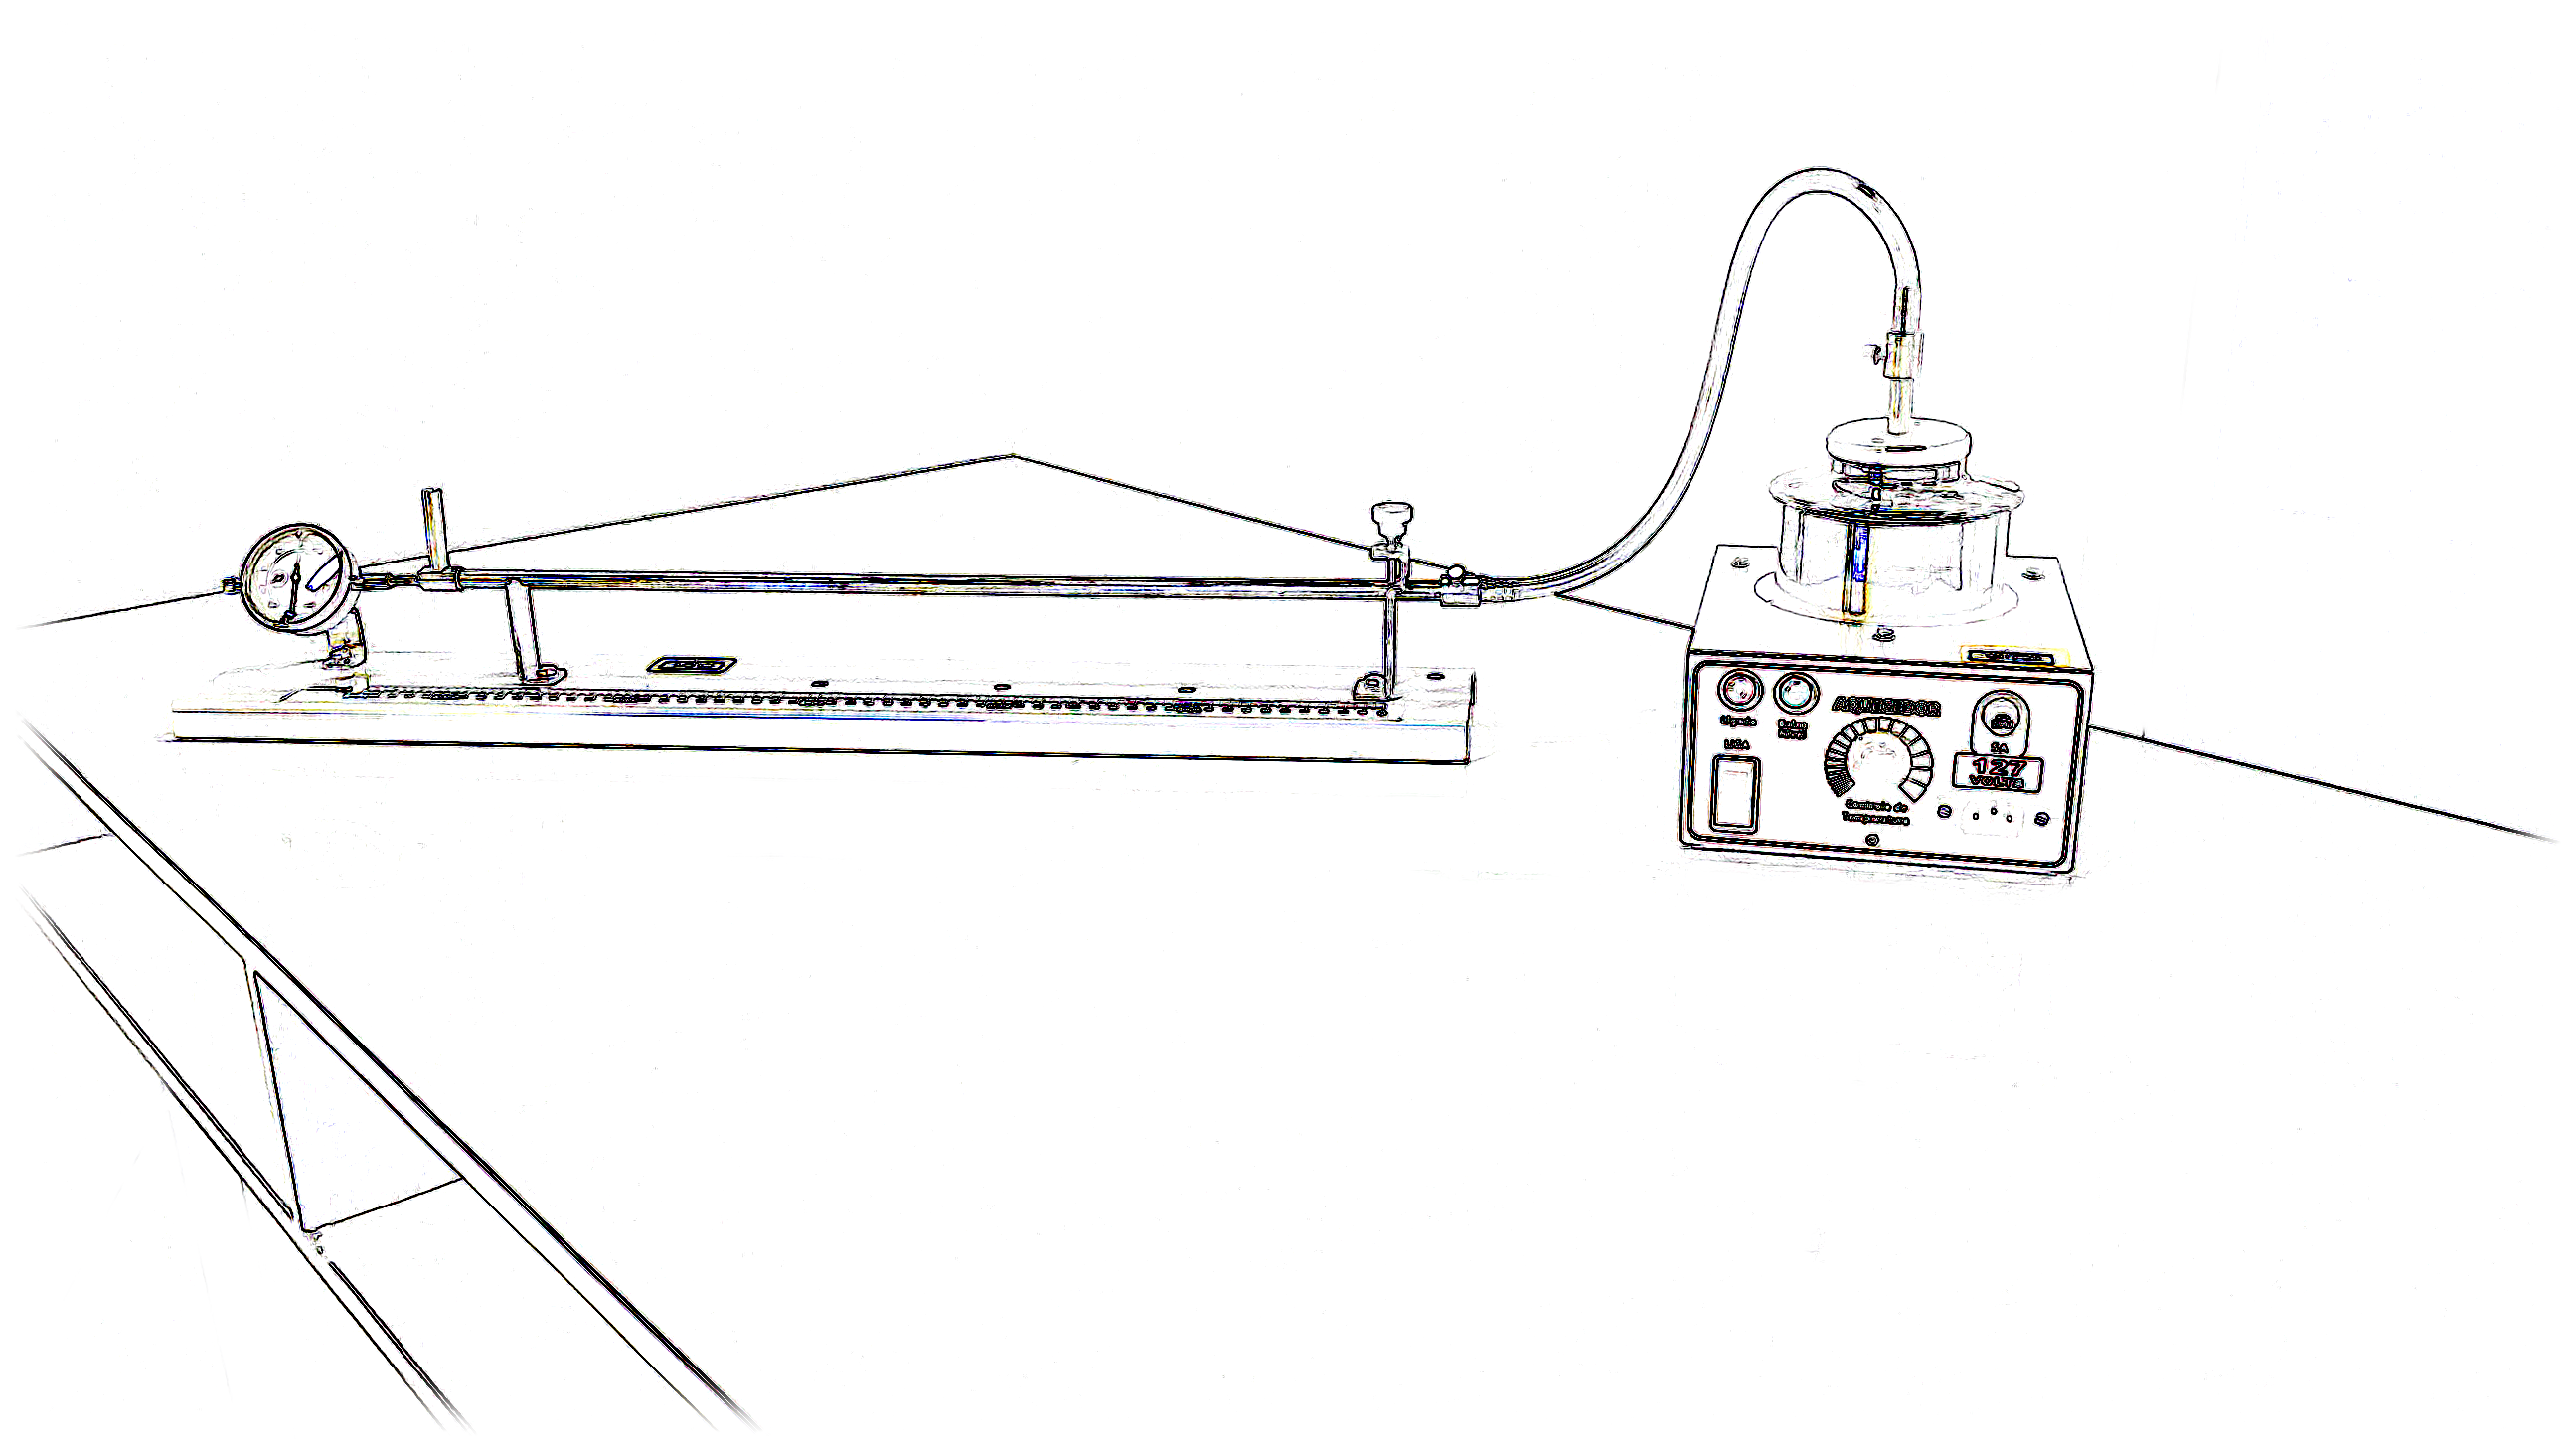
\includegraphics[width=\textwidth]{Ilustrations/Dilatacao.png}
\caption{Equipamento para a verificação experimental da dilatação linear de sólidos.}
\end{figure}
%%%%%%%%%%%%%%%%%%%%%%%%%%%%%%%%%%%%%%%%%%%%%%%%%%%%%%%%%%%%%%%%%%%%%%%%%%%%%%%
\section{Lei de resfriamento de Newton}
%%%%%%%%%%%%%%%%%%%%%%%%%%%%%%%%%%%%%%%%%%%%%%%%%%%%%%%%%%%%%%%%%%%%%%%%%%%%%%%
% Caso especial da equação de Fourier para a condução de calor

De acordo com a lei do resfriamento de Newton\footnote{\url{http://www.ugrad.math.ubc.ca/coursedoc/math100/notes/diffeqs/cool.html}}
\begin{quote}\it
	A taxa de variação da temperatura de um corpo é proporcional à diferença entre sua temperatura e a temperatura do ambiente.
\end{quote}
%
Em termos matemáticos podemos descrever a afirmação acima como
\begin{equation}
	\frac{dT}{dt} \propto -(T - T_a),
\end{equation}
%
onde $T$ representa a temperatura do corpo, $dT/dt$ representa a taxa de variação temporal de tal temperatura e $T_a$ representa a temperatura ambiente. O sinal negativo denota o fato de que se $T > T_a$, o corpo sofre uma \emph{diminuição} de sua temperatura, o que significa que $dT/dt < 0$. Podemos escrever a equação acima como uma igualdade com o auxílio de uma constante:
\begin{equation}\label{Eq:VarTIgualKT}
	\frac{dT}{dt} = -k (T - T_a).
\end{equation}

Verificamos que a temperatura $T$ deve ser então uma \emph{função do tempo}, ou seja $T = T(t)$. Podemos encontrar tal função se definirmos
\begin{equation}
	y(t) = T(t) - T_a,
\end{equation}
%
de onde temos que
\begin{equation}
	\frac{dy(t)}{dt} = \frac{dT(t)}{dt} - \frac{dT_a}{dt}.
\end{equation}
%
O segundo termo à direita é zero, pois a temperatura ambiente é constante, portanto
\begin{equation}
	\frac{dy(t)}{dt} = \frac{dT(t)}{dt}.
\end{equation}
%
Substituindo esse resultado e a própria definição de $y(t)$ na Equação~\ref{Eq:VarTIgualKT}, obtemos
\begin{equation}
	\frac{dy(t)}{dt} = -ky(t),
\end{equation}
%
o que pode ser reescrito como
\begin{equation}
	\frac{dy(t)}{y(t)} = -k dt.
\end{equation}

Se imaginarmos que $y(t)$ tem um valor inicial $y(t_i)$ no instante $t_i$ e um valor final $y(t_f)$ em um instante $t_f$, podemos integrar o lado esquerdo entre os valores inicial e final de $y(t)$ e o lado direito entre os valores inicial e final do tempo, obtendo
\begin{equation}
	\int_{y(t_i)}^{y(t_f)} \frac{dy(t)}{y(t)} = -k \int_{t_i}^{t_f} dt,
\end{equation}
%
o que resulta em
\begin{equation}\label{Eq:TempFuncTempoLN}
	\ln \frac{y(t_f)}{y(t_i)} = - k (t_f - t_i),
\end{equation}
%
onde usamos $\ln \alpha - \ln \beta = \ln (\alpha/\beta)$. Essa equação fica mais simples se fizermos $t_i = 0$, $t_f = t$ e tomarmos a exponencial de ambos os lados da equação:
\begin{equation}
	y(t) = y(0) e^{-kt}.
\end{equation}
%
Finalmente, se notarmos que $y(0) = T(0) - T_a$ e que $T(0)$ é a temperatura inicial $T_0$ do corpo, encontramos
\begin{equation}
	T(t) = T_a + (T_0 - T_a)e^{-kt}.
\end{equation}
%
Temos então que a temperatura do corpo decai segundo uma lei \emph{exponencial}, com uma constante característica $k$.
%
\begin{marginfigure}
\centering
\begin{tikzpicture}[>=Stealth,domain=0:4.3]
	\draw[->] (0,0) -- (4.5,0) node[below]{$t$};
	\draw[->] (0,0) -- (0,3.5) node[left]{$T$};
	
	\draw[dashed] (0,1.2) node[left]{$T_a$} -- (4.3,1.2);
	
	\draw[smooth] plot (\x,{1.2 + (2.8 - 1.2) * exp(-0.5 *\x)});
	\draw[smooth] plot (\x,{1.2 + (0.8 - 1.2) * exp(-0.5 *\x)});
	
	\draw (0,2.8) node[left]{$T_1$};
	\draw (0,0.8) node[left]{$T_2$};
\end{tikzpicture}
\caption{Gráfico da temperatura em função do tempo para o resfriamento e para o aquecimento de um corpo segundo a Lei de Newton para o Resfriamento. As temperaturas iniciais são tais que $T_1 > T_a > T_2$, sendo que para $t\to\infty$ as temperaturas $T_1$ e $T_2$ tendem à temperatura ambiente.}
\end{marginfigure}

%%%%%%%%%%%%%%%%%%%%%%%%%
\subsection{Linearização}
%%%%%%%%%%%%%%%%%%%%%%%%%

Voltando à Equação~\ref{Eq:TempFuncTempoLN}, podemos reescrevê-la como
\begin{equation}
	\ln y(t) = -kt + \ln y(0)
\end{equation}
%
onde utilizamos $t_i = 0$. Utilizando a definição de $y(t)$, temos
\begin{equation}
	\ln (T(t) - T_a) = - kt + \ln(T_0 - T_a).
\end{equation}
%
Comparando essa equação com a equação da reta, temos
\begin{subequations}\label{Eq:LinResfriamentoNewton}
\begin{align}
	y &= \ln (T(t) - T_a) \\
	x &= t \\
	B &= -k \\
	A &= \ln(T_0 - T_a).
\end{align}
\end{subequations}
%
Portanto, podemos determinar o valor de $k$ a partir de uma regressão linear.

%%%%%%%%%%%%%%%%%%%%%%%%%%%%%%%%%%%%%%%%%%%%%%%%%%%%%%%%%%%%%%%%%%%%%%%%%%%%%%%
\section{Experimento}
%%%%%%%%%%%%%%%%%%%%%%%%%%%%%%%%%%%%%%%%%%%%%%%%%%%%%%%%%%%%%%%%%%%%%%%%%%%%%%%

Vamos aquecer tubos metálicos em forma de L através de um fluxo de vapor d'água. Como o tubo estará preso próximo da extremidade de sua lateral maior, verificaremos uma leitura no dilatômetro disposto em contato com a extremidade livre. Após isso, cessaremos o fluxo de vapor, permitindo que o tubo inicie um processo de resfriamento. Durante o resfriamento, monitoraremos a leitura do dilatômetro, que registrará o encolhimento do tubo, bem como de sua temperatura.

%%%%%%%%%%%%%%%%%%%%%%
\subsection{Objetivos}
\label{Sec:ObjetivosDilatacaoLinear}
%%%%%%%%%%%%%%%%%%%%%%

\begin{enumerate}
	\item Verificar a lineariedade da relação entre o comprimento de barras metálicas de diferentes materiais e a variação da temperatura.
	\item Calcular o coeficiente de expansão térmica para o material das barras identificando o material da barra com base em tal propriedade.
	\item Verificar o decaimento exponencial da temperatura, de acordo com a lei do resfriamento de Newton.
	\item Determinar o valor de $k$ para cada uma das barras.
\end{enumerate}

%%%%%%%%%%%%%%%%%%%%%%%%%%%%%%%%%%%%%%%%%%%%%%%%%%%%%%%%%%%%%%%%%%%%%%%%%%%%%%%
\section{Material Necessário}
%%%%%%%%%%%%%%%%%%%%%%%%%%%%%%%%%%%%%%%%%%%%%%%%%%%%%%%%%%%%%%%%%%%%%%%%%%%%%%%

\begin{itemize}
	\item Tubos metálicos em forma de L;
	\item Aquecedor elétrico de água;
	\item Termômetro;
	\item Régua;
	\item Aparato para medição de dilatações térmicas lineares;
	\item Cronômetro.
\end{itemize}

%%%%%%%%%%%%%%%%%%%%%%%%%%%%%%%%%%%%%%%%%%%%%%%%%%%%%%%%%%%%%%%%%%%%%%%%%%%%%%%
\section{Procedimento Experimental}
%%%%%%%%%%%%%%%%%%%%%%%%%%%%%%%%%%%%%%%%%%%%%%%%%%%%%%%%%%%%%%%%%%%%%%%%%%%%%%%
\begin{marginfigure}
	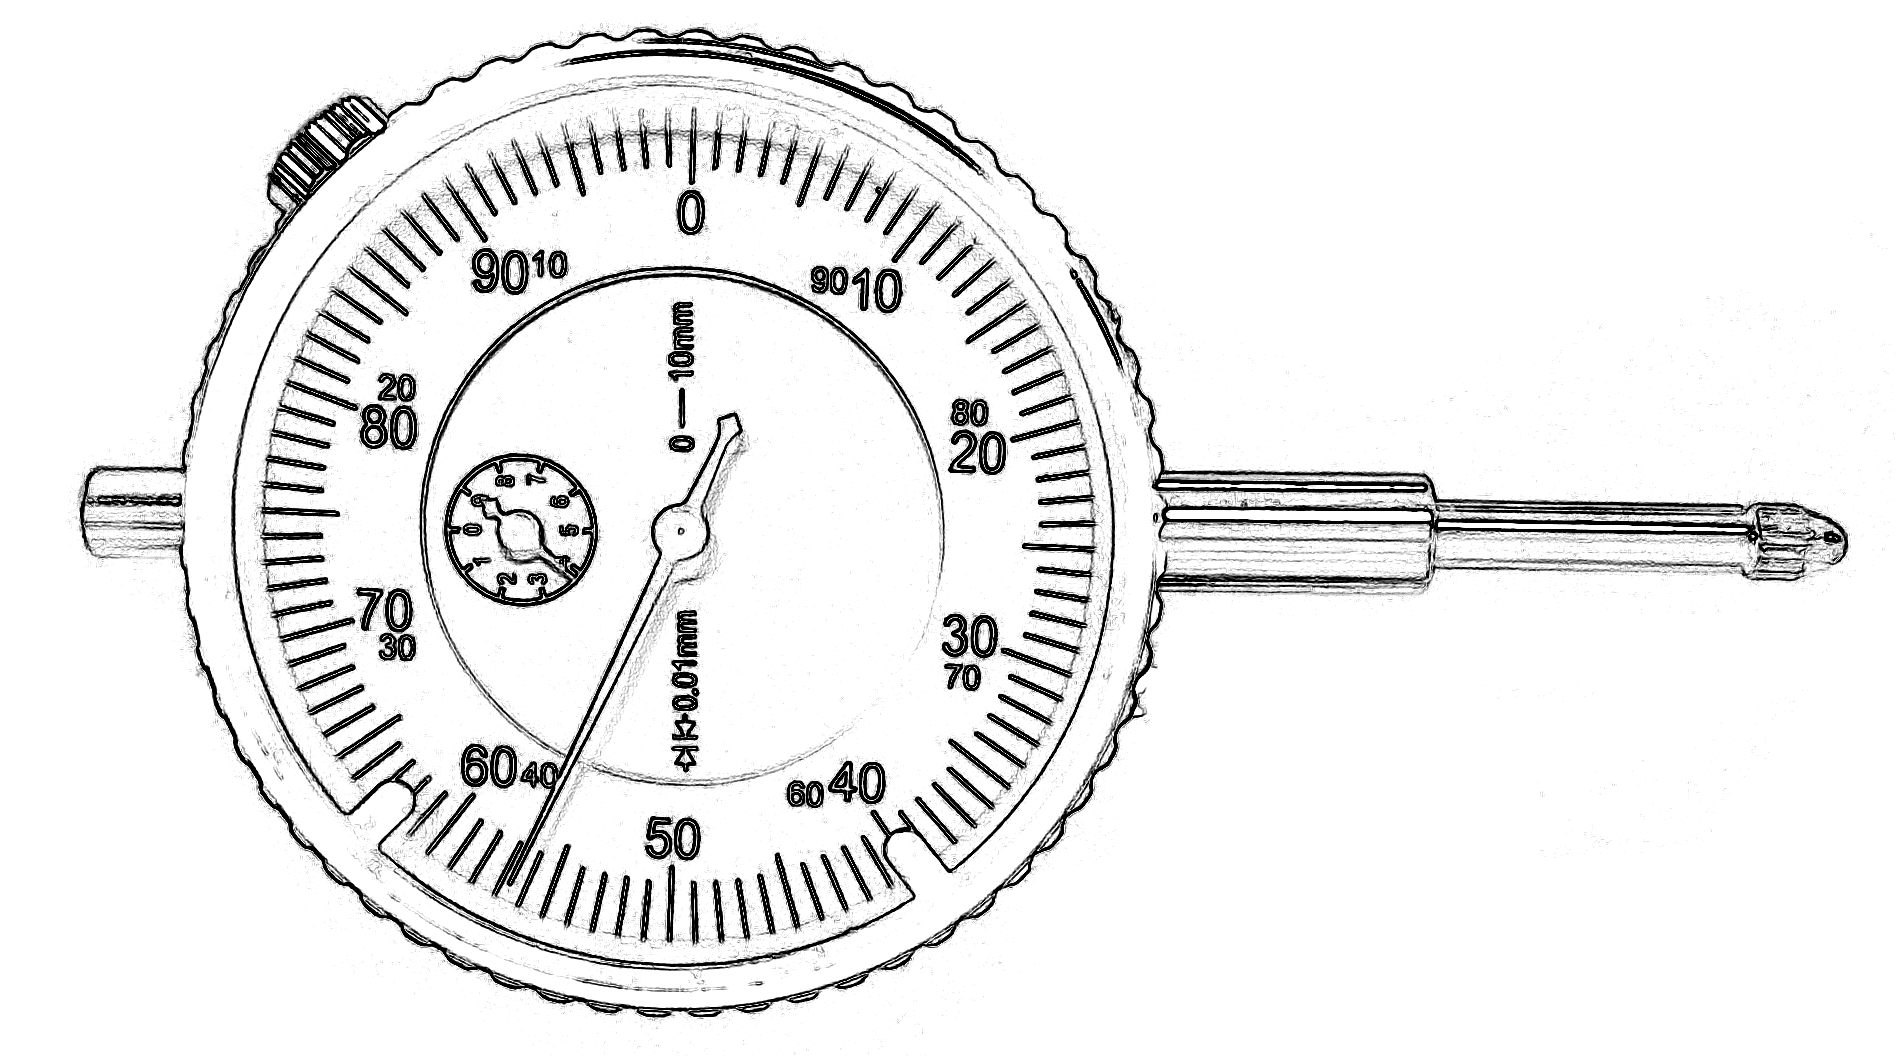
\includegraphics[width=\textwidth]{Ilustrations/Dilatometro.png}
	\caption{Dilatômetro. Note a existência de números pequenos para facilitar a leitura nos casos em que ocorre uma diminuição de tamanho. A coroa externa pode ser girada para zerar o dilatômetro, bastando para isso soltar o parafuso superior.}
\end{marginfigure}

\begin{enumerate}
\item Coloque o tubo metálico com a extremidade em forma de L em contato com o dilatômetro, com o segmento menor disposto verticalmente para cima.
\item Posicione a extremidade do tubo de forma que ela pressione o pino do dilatômetro e fique a uma distância de aproximadamente \np[mm]{520,0} do parafuso de fixação (utilize a escala milimetrada do suporte). Prenda a outra extremidade do tubo utilizando o parafuso do suporte.
\item Prenda a mangueira do aquecedor à extremidade horizontal do tubo (aquela oposta ao dilatômetro).
\item Adicione água ao aquecedor até uma profundidade de aproximadamente \np[cm]{5,0}. \emph{Importante: o aquecedor não pode ficar sem água durante o experimento, pois isso pode causar um superaquecimento e a consequente queima do aparelho.}
\item Ligue o aquecedor e aguarde  até que a água ferva.
\item Quando a água ferver, o tubo dilatará. Quando ele parar de dilatar, coloque o termômetro na extremidade do tubo mais próxima do dilatômetro e aguarde até que sua temperatura pare de variar.
\item Utilizando a régua ou a escala do suporte, meça o comprimento $L_0$ da barra entre o parafuso de fixação e a extremidade próxima ao dilatômetro. Anote este valor na Tabela~\ref{Tab:DadosTubo1}.
\item Anote também a temperatura $T_0$ indicada pelo termômetro.
\item Zere o dilatômetro girando a coroa exterior.
\item Zere o cronômetro.
\item Desligue o aquecedor e aguarde até que o ponteiro do dilatômetro passe a se mover\footnote{Veja que o dilatômetro sofre uma variação negativa, pois a barra está encolhendo. Faça a leitura nos números pequenos do mostrador.}. Assim que ele o fizer, inicie o cronômetro.
\item Quando a temperatura atingir \np[\tcdegree]{90}, faça a leitura do dilatômetro e do cronômetro e anote na Tabela~\ref{Tab:DadosTubo1}.
\item Faça a leitura do dilatômetro e do cronômetro a cada \np[\tcdegree C]{5,0} perdidos. Anote os valores na Tabela~\ref{Tab:DadosTubo1}, incluindo a temperatura. Cesse a leitura quando a temperatura do tubo estiver a aproximadamente \np[\tcdegree]{15,0} acima da temperatura ambiente.
\item Repita o procedimento para os outros tubos e anote os dados nas Tabelas~\ref{Tab:DadosTubo2} e~\ref{Tab:DadosTubo3}.
\end{enumerate}

%%%%%%%%%%%%%%%%%%%%%%%%%%%%%%%%%%%%%%%%%%%%%%%%%%%%%%%%%%%%%%%%%%%%%%%%%%%%%%%
%%%%%%%%%%%%%%%%%%%%%%%%%%%%%%%%%%%%%%%%%%%%%%%%%%%%%%%%%%%%%%%%%%%%%%%%%%%%%%%
%%%%%%%%%%%%%%%%%%%%%%%%%%%%%%%%%%%%%%%%%%%%%%%%%%%%%%%%%%%%%%%%%%%%%%%%%%%%%%%
%%%%%%%%%%%%%%%%%%%%%%%%%%%%%%%%%%%%%%%%%%%%%%%%%%%%%%%%%%%%%%%%%%%%%%%%%%%%%%%
\cleardoublepage

\noindent{}{\huge\textit{Dilatação linear e lei de resfriamento de Newton}}

\vspace{15mm}

\begin{fullwidth}
\noindent{}\makebox[0.6\linewidth]{Turma:\enspace\hrulefill}\makebox[0.4\textwidth]{  Data:\enspace\hrulefill}
\vspace{5mm}

\noindent{}\makebox[0.6\linewidth]{Aluno(a):\enspace\hrulefill}\makebox[0.4\textwidth]{  Matrícula:\enspace\hrulefill}

\noindent{}\makebox[0.6\linewidth]{Aluno(a):\enspace\hrulefill}\makebox[0.4\textwidth]{  Matrícula:\enspace\hrulefill}

\noindent{}\makebox[0.6\linewidth]{Aluno(a):\enspace\hrulefill}\makebox[0.4\textwidth]{  Matrícula:\enspace\hrulefill}

\noindent{}\makebox[0.6\linewidth]{Aluno(a):\enspace\hrulefill}\makebox[0.4\textwidth]{  Matrícula:\enspace\hrulefill}

\noindent{}\makebox[0.6\linewidth]{Aluno(a):\enspace\hrulefill}\makebox[0.4\textwidth]{  Matrícula:\enspace\hrulefill}
\end{fullwidth}

\vspace{5mm}

%%%%%%%%%%%%%%%%%%%%%%%%%%%%%%%%%%%%%%%%%%%%%%%%%%%%%%%%%%%%%%%%%%%%%%%%%%%%%%%
\section{Questionário}
%%%%%%%%%%%%%%%%%%%%%%%%%%%%%%%%%%%%%%%%%%%%%%%%%%%%%%%%%%%%%%%%%%%%%%%%%%%%%%%

\begin{question}[type={exam}]{1}
Apresente os resultados de maneira clara e organizada. Mostre os cálculos requisitados de maneira clara e sucinta, evidenciando o raciocínio desenvolvido.
\end{question}

\begin{question}[type={exam}]{0.5}
Liste os equipamentos utilizados. Para os instrumentos de medida, descreva o tipo do equipamento, sua resolução, e seu erro de escala.
\end{question}

\begin{question}[type={exam}]{0.5}
Preencha as tabelas com o número adequado de algarismos significativos, unidades, e erros de escala apropriados. 
\end{question}

\begin{question}[type={exam}]{1.0}
Elabore um gráfico\footnote{Os três conjuntos de dados devem ser representados no mesmo gráfico, possibilitando a comparação entre eles. Note ainda que o gráfico será decrescente, uma vez que estamos verificando o processo de encolhimento das barras conforme elas resfriam.} de $L \times |T - T_0|$ com os dados das Tabelas~\ref{Tab:DadosTubo1}, \ref{Tab:DadosTubo2} e~\ref{Tab:DadosTubo3}.
\end{question}

\begin{question}[type={exam}]{0.5}
Para a questão anterior, calcule as retas que melhor representam os dados experimentais utilizando o método dos mínimos quadrados e as adicione ao gráfico.
\end{question}
 
\begin{question}[type={exam}]{1}
Calcule o valor do coeficiente de expansão térmica para os materiais através dos coeficientes angulares e lineares obtidos na questão anterior. Identifique os materiais utilizando os dados da Tabela~\ref{TabelaCoeficientes} e calcule o erro percentual obtido através da expressão
\begin{equation}
	E_{\%} = \left|\frac{x-x_{\textrm{ref}}}{x_{\textrm{ref}}}\right| \times 100.
\end{equation}
\end{question}

\begin{question}[type={exam}]{1}
Para os dados da Tabela~\ref{Tab:DadosTubo1}, calcule o erro associado às constantes $A$ e $B$ e determine o erro associado ao coeficiente de expansão térmica.
\end{question}

\begin{question}[type={exam}]{1}
Elabore um gráfico de $T \times t$ para os dados das  Tabelas~\ref{Tab:DadosTubo1}, \ref{Tab:DadosTubo2} e~\ref{Tab:DadosTubo3}.
\end{question}

\begin{question}[type={exam}]{1}
Elabore um gráfico linearizado de acordo com o conjunto de Equações~\eqref{Eq:LinResfriamentoNewton} para os dados das  Tabelas~\ref{Tab:DadosTubo1}, \ref{Tab:DadosTubo2} e~\ref{Tab:DadosTubo3}.
\end{question}

\begin{question}[type={exam}]{1}
Para a questão anterior, calcule as melhores retas através do método de mínimos quadrados e as adicione ao gráfico linearizado. Calcule os valores da constante $k$ através dos coeficientes angulares.
\end{question}

\begin{question}[type={exam}]{1.5}
Considerando os objetivos do experimento, listados na Seção~\ref{Sec:ObjetivosDilatacaoLinear}, e os resultados obtidos nas questões anteriores, discuta quais objetivos foram atingidos com sucesso, justificando suas conclusões. Se algum objetivo não foi atingido, discuta quais são os possíveis motivos do fracasso e que providências podem ser tomadas para que eles sejam alcançados.
\end{question}

\vfill
%%%%%%%%%%%%%%%%%%%%%%%%%%%%%%%%%%%%%%%%%%%%%%%%%%%%%%%%%%%%%%%%%%%%%%%%%%%%%%%
\pagebreak
\section{Tabelas}
%%%%%%%%%%%%%%%%%%%%%%%%%%%%%%%%%%%%%%%%%%%%%%%%%%%%%%%%%%%%%%%%%%%%%%%%%%%%%%%
\begin{table*}[!ht]
\caption[][1cm]{Dados para a dilatação do Tubo 1.}
\label{Tab:DadosTubo1}
\centering
	\begin{tabular}{lllll}
		\toprule
		&\textbf{Dados Iniciais}\\
		\cmidrule{2-3}
		& \cellcolor[gray]{0.89}$L_0$ &\cellcolor[gray]{0.92}\\
		& \cellcolor[gray]{0.95}$T_0$ & \cellcolor[gray]{0.97}\\
		& \cellcolor[gray]{0.89}$T_a$ & \cellcolor[gray]{0.92}\\
		\cmidrule{2-3}
\\
		&\multicolumn{3}{l}{\textbf{Dados para o resfriamento}} \\
		\cmidrule{2-4}
		& $T$ & $\Delta L$ & t &\\
		\cmidrule{2-4}
		& \cellcolor[gray]{0.89} \phantom{xxxxxxxxxxxxxxxxxxxx}& \cellcolor[gray]{0.92} \phantom{xxxxxxxxxxxxxxxxxxxx} &  \cellcolor[gray]{0.89} \phantom{xxxxxxxxxxxxxxxxxxxx} \\
		& \cellcolor[gray]{0.95} & \cellcolor[gray]{0.97} & \cellcolor[gray]{0.95} \\
		& \cellcolor[gray]{0.89} & \cellcolor[gray]{0.92} & \cellcolor[gray]{0.89} \\
		& \cellcolor[gray]{0.95} & \cellcolor[gray]{0.97} & \cellcolor[gray]{0.95} \\
		& \cellcolor[gray]{0.89} & \cellcolor[gray]{0.92} & \cellcolor[gray]{0.89} \\
		& \cellcolor[gray]{0.95} & \cellcolor[gray]{0.97} & \cellcolor[gray]{0.95} \\
		& \cellcolor[gray]{0.89} & \cellcolor[gray]{0.92} & \cellcolor[gray]{0.89} \\
		& \cellcolor[gray]{0.95} & \cellcolor[gray]{0.97} & \cellcolor[gray]{0.95} \\
		& \cellcolor[gray]{0.89} & \cellcolor[gray]{0.92} & \cellcolor[gray]{0.89} \\
		& \cellcolor[gray]{0.95} & \cellcolor[gray]{0.97} & \cellcolor[gray]{0.95} \\
		& \cellcolor[gray]{0.89} & \cellcolor[gray]{0.92} & \cellcolor[gray]{0.89} \\
		& \cellcolor[gray]{0.95} & \cellcolor[gray]{0.97} & \cellcolor[gray]{0.95} \\
		& \cellcolor[gray]{0.89} & \cellcolor[gray]{0.92} & \cellcolor[gray]{0.89} \\
		& \cellcolor[gray]{0.95} & \cellcolor[gray]{0.97} & \cellcolor[gray]{0.95} \\
		& \cellcolor[gray]{0.89} & \cellcolor[gray]{0.92} & \cellcolor[gray]{0.89} \\
		& \cellcolor[gray]{0.95} & \cellcolor[gray]{0.97} & \cellcolor[gray]{0.95} \\
		\cmidrule{2-4}
\\
		&\multicolumn{3}{l}{\textbf{Dados para elaboração dos gráficos}} \\
		\cmidrule{2-4}
		& $L$ & $T - T_0$ & $T - T_a$ \\
		\cmidrule{2-4}
		& \cellcolor[gray]{0.89} & \cellcolor[gray]{0.92} & \cellcolor[gray]{0.89} \\
		& \cellcolor[gray]{0.95} & \cellcolor[gray]{0.97} & \cellcolor[gray]{0.95} \\
		& \cellcolor[gray]{0.89} & \cellcolor[gray]{0.92} & \cellcolor[gray]{0.89} \\
		& \cellcolor[gray]{0.95} & \cellcolor[gray]{0.97} & \cellcolor[gray]{0.95} \\
		& \cellcolor[gray]{0.89} & \cellcolor[gray]{0.92} & \cellcolor[gray]{0.89} \\
		& \cellcolor[gray]{0.95} & \cellcolor[gray]{0.97} & \cellcolor[gray]{0.95} \\
		& \cellcolor[gray]{0.89} & \cellcolor[gray]{0.92} & \cellcolor[gray]{0.89} \\
		& \cellcolor[gray]{0.95} & \cellcolor[gray]{0.97} & \cellcolor[gray]{0.95} \\
		& \cellcolor[gray]{0.89} & \cellcolor[gray]{0.92} & \cellcolor[gray]{0.89} \\
		& \cellcolor[gray]{0.95} & \cellcolor[gray]{0.97} & \cellcolor[gray]{0.95} \\
		& \cellcolor[gray]{0.89} & \cellcolor[gray]{0.92} & \cellcolor[gray]{0.89} \\
		& \cellcolor[gray]{0.95} & \cellcolor[gray]{0.97} & \cellcolor[gray]{0.95} \\
		& \cellcolor[gray]{0.89} & \cellcolor[gray]{0.92} & \cellcolor[gray]{0.89} \\
		& \cellcolor[gray]{0.95} & \cellcolor[gray]{0.97} & \cellcolor[gray]{0.95} \\
		& \cellcolor[gray]{0.89} & \cellcolor[gray]{0.92} & \cellcolor[gray]{0.89} \\
		& \cellcolor[gray]{0.95} & \cellcolor[gray]{0.97} & \cellcolor[gray]{0.95} \\
		\bottomrule
	\end{tabular}
\end{table*}

\begin{table*}[!ht]
\forceversofloat
\caption[][1cm]{Dados para a dilatação do Tubo 2.}
\label{Tab:DadosTubo2}
\centering
	\begin{tabular}{lllll}
		\toprule
		&\textbf{Dados Iniciais}\\
		\cmidrule{2-3}
		& \cellcolor[gray]{0.89}$L_0$ &\cellcolor[gray]{0.92}\\
		& \cellcolor[gray]{0.95}$T_0$ & \cellcolor[gray]{0.97}\\
		& \cellcolor[gray]{0.89}$T_a$ & \cellcolor[gray]{0.92}\\
		\cmidrule{2-3}
\\
		&\multicolumn{3}{l}{\textbf{Dados para o resfriamento}} \\
		\cmidrule{2-4}
		& $T$ & $\Delta L$ & t &\\
		\cmidrule{2-4}
		& \cellcolor[gray]{0.89} \phantom{xxxxxxxxxxxxxxxxxxxx}& \cellcolor[gray]{0.92} \phantom{xxxxxxxxxxxxxxxxxxxx} &  \cellcolor[gray]{0.89} \phantom{xxxxxxxxxxxxxxxxxxxx} \\
		& \cellcolor[gray]{0.95} & \cellcolor[gray]{0.97} & \cellcolor[gray]{0.95} \\
		& \cellcolor[gray]{0.89} & \cellcolor[gray]{0.92} & \cellcolor[gray]{0.89} \\
		& \cellcolor[gray]{0.95} & \cellcolor[gray]{0.97} & \cellcolor[gray]{0.95} \\
		& \cellcolor[gray]{0.89} & \cellcolor[gray]{0.92} & \cellcolor[gray]{0.89} \\
		& \cellcolor[gray]{0.95} & \cellcolor[gray]{0.97} & \cellcolor[gray]{0.95} \\
		& \cellcolor[gray]{0.89} & \cellcolor[gray]{0.92} & \cellcolor[gray]{0.89} \\
		& \cellcolor[gray]{0.95} & \cellcolor[gray]{0.97} & \cellcolor[gray]{0.95} \\
		& \cellcolor[gray]{0.89} & \cellcolor[gray]{0.92} & \cellcolor[gray]{0.89} \\
		& \cellcolor[gray]{0.95} & \cellcolor[gray]{0.97} & \cellcolor[gray]{0.95} \\
		& \cellcolor[gray]{0.89} & \cellcolor[gray]{0.92} & \cellcolor[gray]{0.89} \\
		& \cellcolor[gray]{0.95} & \cellcolor[gray]{0.97} & \cellcolor[gray]{0.95} \\
		& \cellcolor[gray]{0.89} & \cellcolor[gray]{0.92} & \cellcolor[gray]{0.89} \\
		& \cellcolor[gray]{0.95} & \cellcolor[gray]{0.97} & \cellcolor[gray]{0.95} \\
		& \cellcolor[gray]{0.89} & \cellcolor[gray]{0.92} & \cellcolor[gray]{0.89} \\
		& \cellcolor[gray]{0.95} & \cellcolor[gray]{0.97} & \cellcolor[gray]{0.95} \\
		\cmidrule{2-4}
\\
		&\multicolumn{3}{l}{\textbf{Dados para elaboração dos gráficos}} \\
		\cmidrule{2-4}
		& $L$ & $T - T_0$ & $T - T_a$ \\
		\cmidrule{2-4}
		& \cellcolor[gray]{0.89} & \cellcolor[gray]{0.92} & \cellcolor[gray]{0.89} \\
		& \cellcolor[gray]{0.95} & \cellcolor[gray]{0.97} & \cellcolor[gray]{0.95} \\
		& \cellcolor[gray]{0.89} & \cellcolor[gray]{0.92} & \cellcolor[gray]{0.89} \\
		& \cellcolor[gray]{0.95} & \cellcolor[gray]{0.97} & \cellcolor[gray]{0.95} \\
		& \cellcolor[gray]{0.89} & \cellcolor[gray]{0.92} & \cellcolor[gray]{0.89} \\
		& \cellcolor[gray]{0.95} & \cellcolor[gray]{0.97} & \cellcolor[gray]{0.95} \\
		& \cellcolor[gray]{0.89} & \cellcolor[gray]{0.92} & \cellcolor[gray]{0.89} \\
		& \cellcolor[gray]{0.95} & \cellcolor[gray]{0.97} & \cellcolor[gray]{0.95} \\
		& \cellcolor[gray]{0.89} & \cellcolor[gray]{0.92} & \cellcolor[gray]{0.89} \\
		& \cellcolor[gray]{0.95} & \cellcolor[gray]{0.97} & \cellcolor[gray]{0.95} \\
		& \cellcolor[gray]{0.89} & \cellcolor[gray]{0.92} & \cellcolor[gray]{0.89} \\
		& \cellcolor[gray]{0.95} & \cellcolor[gray]{0.97} & \cellcolor[gray]{0.95} \\
		& \cellcolor[gray]{0.89} & \cellcolor[gray]{0.92} & \cellcolor[gray]{0.89} \\
		& \cellcolor[gray]{0.95} & \cellcolor[gray]{0.97} & \cellcolor[gray]{0.95} \\
		& \cellcolor[gray]{0.89} & \cellcolor[gray]{0.92} & \cellcolor[gray]{0.89} \\
		& \cellcolor[gray]{0.95} & \cellcolor[gray]{0.97} & \cellcolor[gray]{0.95} \\
		\bottomrule
	\end{tabular}
\end{table*}

\begin{table*}[!ht]
\caption[][1cm]{Dados para a dilatação do Tubo 3.}
\label{Tab:DadosTubo3}
\centering
	\begin{tabular}{lllll}
		\toprule
		&\textbf{Dados Iniciais}\\
		\cmidrule{2-3}
		& \cellcolor[gray]{0.89}$L_0$ &\cellcolor[gray]{0.92}\\
		& \cellcolor[gray]{0.95}$T_0$ & \cellcolor[gray]{0.97}\\
		& \cellcolor[gray]{0.89}$T_a$ & \cellcolor[gray]{0.92}\\
		\cmidrule{2-3}
\\
		&\multicolumn{3}{l}{\textbf{Dados para o resfriamento}} \\
		\cmidrule{2-4}
		& $T$ & $\Delta L$ & t &\\
		\cmidrule{2-4}
		& \cellcolor[gray]{0.89} \phantom{xxxxxxxxxxxxxxxxxxxx}& \cellcolor[gray]{0.92} \phantom{xxxxxxxxxxxxxxxxxxxx} &  \cellcolor[gray]{0.89} \phantom{xxxxxxxxxxxxxxxxxxxx} \\
		& \cellcolor[gray]{0.95} & \cellcolor[gray]{0.97} & \cellcolor[gray]{0.95} \\
		& \cellcolor[gray]{0.89} & \cellcolor[gray]{0.92} & \cellcolor[gray]{0.89} \\
		& \cellcolor[gray]{0.95} & \cellcolor[gray]{0.97} & \cellcolor[gray]{0.95} \\
		& \cellcolor[gray]{0.89} & \cellcolor[gray]{0.92} & \cellcolor[gray]{0.89} \\
		& \cellcolor[gray]{0.95} & \cellcolor[gray]{0.97} & \cellcolor[gray]{0.95} \\
		& \cellcolor[gray]{0.89} & \cellcolor[gray]{0.92} & \cellcolor[gray]{0.89} \\
		& \cellcolor[gray]{0.95} & \cellcolor[gray]{0.97} & \cellcolor[gray]{0.95} \\
		& \cellcolor[gray]{0.89} & \cellcolor[gray]{0.92} & \cellcolor[gray]{0.89} \\
		& \cellcolor[gray]{0.95} & \cellcolor[gray]{0.97} & \cellcolor[gray]{0.95} \\
		& \cellcolor[gray]{0.89} & \cellcolor[gray]{0.92} & \cellcolor[gray]{0.89} \\
		& \cellcolor[gray]{0.95} & \cellcolor[gray]{0.97} & \cellcolor[gray]{0.95} \\
		& \cellcolor[gray]{0.89} & \cellcolor[gray]{0.92} & \cellcolor[gray]{0.89} \\
		& \cellcolor[gray]{0.95} & \cellcolor[gray]{0.97} & \cellcolor[gray]{0.95} \\
		& \cellcolor[gray]{0.89} & \cellcolor[gray]{0.92} & \cellcolor[gray]{0.89} \\
		& \cellcolor[gray]{0.95} & \cellcolor[gray]{0.97} & \cellcolor[gray]{0.95} \\
		\cmidrule{2-4}
\\
		&\multicolumn{3}{l}{\textbf{Dados para elaboração dos gráficos}} \\
		\cmidrule{2-4}
		& $L$ & $T - T_0$ & $T - T_a$ \\
		\cmidrule{2-4}
		& \cellcolor[gray]{0.89} & \cellcolor[gray]{0.92} & \cellcolor[gray]{0.89} \\
		& \cellcolor[gray]{0.95} & \cellcolor[gray]{0.97} & \cellcolor[gray]{0.95} \\
		& \cellcolor[gray]{0.89} & \cellcolor[gray]{0.92} & \cellcolor[gray]{0.89} \\
		& \cellcolor[gray]{0.95} & \cellcolor[gray]{0.97} & \cellcolor[gray]{0.95} \\
		& \cellcolor[gray]{0.89} & \cellcolor[gray]{0.92} & \cellcolor[gray]{0.89} \\
		& \cellcolor[gray]{0.95} & \cellcolor[gray]{0.97} & \cellcolor[gray]{0.95} \\
		& \cellcolor[gray]{0.89} & \cellcolor[gray]{0.92} & \cellcolor[gray]{0.89} \\
		& \cellcolor[gray]{0.95} & \cellcolor[gray]{0.97} & \cellcolor[gray]{0.95} \\
		& \cellcolor[gray]{0.89} & \cellcolor[gray]{0.92} & \cellcolor[gray]{0.89} \\
		& \cellcolor[gray]{0.95} & \cellcolor[gray]{0.97} & \cellcolor[gray]{0.95} \\
		& \cellcolor[gray]{0.89} & \cellcolor[gray]{0.92} & \cellcolor[gray]{0.89} \\
		& \cellcolor[gray]{0.95} & \cellcolor[gray]{0.97} & \cellcolor[gray]{0.95} \\
		& \cellcolor[gray]{0.89} & \cellcolor[gray]{0.92} & \cellcolor[gray]{0.89} \\
		& \cellcolor[gray]{0.95} & \cellcolor[gray]{0.97} & \cellcolor[gray]{0.95} \\
		& \cellcolor[gray]{0.89} & \cellcolor[gray]{0.92} & \cellcolor[gray]{0.89} \\
		& \cellcolor[gray]{0.95} & \cellcolor[gray]{0.97} & \cellcolor[gray]{0.95} \\
		\bottomrule
	\end{tabular}
\end{table*}


